\documentclass[12pt]{article}
\usepackage[shortlabels]{enumitem}
\usepackage{graphicx}
\begin{document}
\title{TCSS 343 - Week 4}
\author{Jake McKenzie}
\maketitle
\noindent\centerline{\textbf{Homework 2}}
\\\\2.10 Why do some systems store the operating system in firmware, while
others store it on disk?\\\\
\textbf{ANSWER: }Embedded devices are typically smaller, many would
like to have to map ROM directly to memory. As such they have no need 
for a file system or any of niceties that go along with systems that 
store the OS on disk. The gameboy is an example of such an embedded 
device. This gameboy would map ROM directly to memory, storing the 
OS in firmware. To change the OS on the gameboy you would need to flash 
the firmware. 
\\\\2.16 What are the advantages and disadvantages of using the same 
systemcall interface for manipulating both files and devices?\\\\
\textbf{ANSWER: }A major advantage of interoperability between 
using the same systemcall interface for manipulating both 
files and devices is allowing for a higher level of abstraction.
This abstraction leads to less code re-use. A major disadvantage 
of this is the potential to lose performance, but this is a 
disadvantage that is harder to pin down. Whenever you add any 
layer of abstraction to a system you include the potnetial for 
the loss of functionality or performance. That said, I think 
the advantage of say, UNIX's ability to treat hardware devices 
as files is a major advantage outweighing most disadvantages.
\\\\2.18 What are the two models of interprocess communication? What 
are the strengths and weaknesses of the two approaches?\\\\
\textbf{ANSWER: }The two models of interprocess communication 
are the message-passing model and the shared-memory model. 
Since message-passing is a system call, it has a slightly 
higher overhead than shared-memory model. This lack of system 
calls on the other hand mean than it takes more overhead from
the programmer to take care of how the memory is shared.
\\\\2.19 Why is the separation of mechanism and policy desirable?\\\\
\textbf{ANSWER: }If there was no separation between the mechanism 
and policy the system would lack the resililence to implement the 
functionalities that are desirable in a computing system. The book 
gives a timer as an example of a mechanism which ensures CPU 
protection, the decision that decides how long the timer is 
to be set for are particular user is a policy decision. I didn't 
like this example. I think a working directory (unix) or ``context 
sensitive addressing'' is a mechanism which references a 
different object depending upon the context in which the 
address is used, but the decision as to how this protection 
is implemented is dependent on each particular user, especially in 
Linux but also true for many other operating systems. I don't know 
if this works but I would rather attempt to answer the question without 
regurgitating what the book is telling me, but apply what the 
book is telling in some way.
\\\\2.21 What is the main advantage of the microkernel approach to system
design? How do user programs and system services interact in a
microkernel architecture? What are the disadvantages of using the
microkernel approach?\\\\
\textbf{ANSWER: }The main advantage of the microkernel approach 
is that when you add some new service in the operating system that 
does not modify the kernel. Like a government that rules a nation 
and all its states, the kernel is the central set of instructions 
that not only governs how processes interact with the body politic 
but also provides the rules on how they should use the institutions 
in the computing device, such as the disk, the memory or I/O devices.
Like any good government it should be hard to change the core 
institutions, which is where the microkernel comes in.\\\\
Programs that manage each individual I/O device, for example, 
are the staff which keep all the departments which use these I/O 
device of the OS running smoothing. Communication through message 
passing and shared memory(not mentioned in the book but I believe 
is also true) is the main function of the microkernel. This, I believe, 
is what leads to what you mentioned in class of having for example
 ``good mixture of different heavy CPU intensive tasks 
and I/O tasks''.\\\\
By introducing microkernels you can suffer from performance decreases 
due to the inflation of system function overhead that comes with 
more microkernels.\\\\
2.22 What are the advantages of using loadable kernel modules?\\\\
\textbf{ANSWER: }Loading kernel modules are ideal of adding/removing code to/from 
the kernel at runtime, ideal for device drivers, reducing the size of 
the kernel, and are especially used in linux as it is a monolithic kernal.
One of the major ways to add functionality to linux is through LKMs for 
this reason.
\\\\
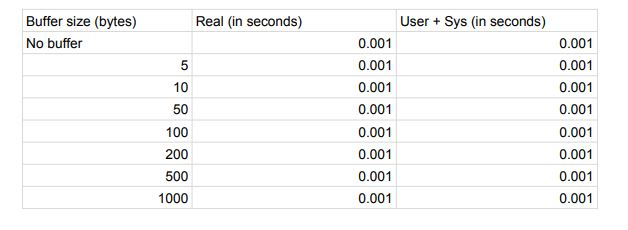
\includegraphics{table.jpg}\\
(I have a very fast PC and this is a new light install of the OS of 
Ubuntu. I thought about downloading a bigger book to show the 
differences but you didn't ask for one. If this is a problem 
I can resubmit for you. I think I get the point you were 
trying to make.)
\end{document}